\documentclass[preprint,12pt]{elsarticle}

\usepackage{amsmath,amssymb,bm}
\usepackage{booktabs}
\usepackage{graphicx}
\usepackage{multirow}
\usepackage{array}
\usepackage{lineno}
\usepackage{setspace}
\usepackage{hyperref}
\usepackage{caption}
\usepackage{subcaption}
\usepackage{threeparttable}

\journal{Pattern Recognition}
\biboptions{sort&compress}
\graphicspath{{figures/}}
\doublespacing
\linenumbers

\newcommand{\Dice}{\operatorname{Dice}}
\newcommand{\EDT}{\operatorname{EDT}}
\newcommand{\I}{\mathcal{I}}
\newcommand{\Yp}{Y_{\mathrm{p}}}
\newcommand{\Ygt}{Y_{\mathrm{gt}}}
\newcommand{\Yfinal}{Y_{\mathrm{final}}}
\newcommand{\ROAR}{R_{\mathrm{OAR}}}

\begin{document}

\begin{highlights}
\item Sparse target prompts are converted into structured 3D pseudo-labels.
\item Distance-field core-envelope priors constrain target completion.
\item A residual 3D U-Net learns supervised pseudo-to-true correction.
\item Refinement improves test Dice from 0.9278 to 0.9341.
\item Paired testing confirms significant gain over the pseudo-label.
\end{highlights}


\begin{frontmatter}

\title{Organ-at-Risk-Constrained Sparse-Prompt Clinical Target Volume Completion with Supervised Pseudo-to-True Refinement}

\author[inst1]{Yanxin Huang}
\ead{corresponding.email@institution.edu}

\affiliation[inst1]{
  organization={Institution to be finalized},
  city={City},
  country={Country}
}

\begin{abstract}
Clinical target volume (CTV) delineation in radiotherapy is difficult to automate because the target is not a directly visible object and depends on anatomy, margin rules, sparse clinician intent, and physician-specific contouring habits. We study CTV delineation as a biomedical data preprocessing problem: transforming a small number of clinician-approved two-dimensional CTV slices into an auditable three-dimensional pseudo-label and then refining it with a supervised pseudo-to-true correction network. The workflow uses planning CT, organ-at-risk (OAR) masks, and $K=7$ sparse CTV slice prompts. Signed distance function (SDF) propagation first constructs a high-precision core, high-recall envelope, and support-intersection pseudo-label. A lightweight residual 3D U-Net then learns a supervised correction from pseudo-label to expert CTV, conditioned on CT, OAR-derived anatomical region of interest, sparse prompts, SDF support, core, envelope, and axial prompt distance. On 31 held-out CTV-positive scans, fully automatic nnU-Net and DiffUNet reach Dice similarity coefficients of $0.400$ and $0.316$, and sparse-prompt SAM-Med3D reaches $0.422$. Same-prompt linear interpolation reaches $0.912$, while the support-intersection pseudo-label reaches $0.9278$. The proposed refine network improves mean Dice to $0.9341$, unseen-slice Dice to $0.9057$, 95th percentile Hausdorff distance (HD95) to $3.11$ mm, and average surface distance (ASD) to $0.84$ mm. Paired testing shows a significant network gain over the input pseudo-label ($\Delta$Dice $=0.0063$, one-sided paired $t$-test $p=3.46\times10^{-5}$).
\end{abstract}

\begin{keyword}
Clinical target volume \sep Sparse prompt \sep Data preprocessing \sep Pseudo-label refinement \sep Radiotherapy \sep Medical image segmentation
\end{keyword}

\end{frontmatter}

\section{Introduction}

Clinical target volume (CTV) delineation is a core preprocessing step in radiotherapy planning. In contrast to many organ-at-risk (OAR) segmentation problems, a CTV is not a compact visible structure with a stable boundary. It encodes suspected microscopic extension, clinical margin decisions, anatomical constraints, and physician-specific treatment intent. Volume delineation uncertainty is therefore a known source of radiotherapy variability \cite{vinod2016uncertainties}, and target-volume learning cannot be reduced to ordinary CT-only object segmentation \cite{sharp2014vision,men2021deeptarget}.

This study is positioned under the ``medical data processing'' scope of the Pattern Recognition special issue on multimodal biomedical data. The cohort uses planning CT as the only imaging modality; accordingly, the work is not presented as CT/MRI/PET image-level multimodal fusion. The pattern-recognition problem is instead the integration of heterogeneous biomedical inputs--radiotherapy CT, OAR anatomical masks, sparse clinician annotations, and geometric SDF priors--into a structured preprocessing pipeline for CTV pseudo-label generation and refinement. This distinction is important: the main contribution is not a generic multimodal imaging fusion model, but an auditable data-preprocessing framework for converting sparse clinical intent into a volumetric target label.

Deep segmentation networks such as nnU-Net provide strong automatic baselines across many biomedical tasks \cite{isensee2021nnunet}. Promptable medical segmentation models such as MedSAM and SAM-Med3D extend interactive segmentation to medical images and 3D volumes \cite{ma2024medsam,wang2023sammed3d}. However, our experiments show that fully automatic CT-to-CTV segmentation and generic promptable segmentation remain unstable for this low-contrast, rule-driven CTV task. In this setting, a few complete CTV prompt slices provided by a clinician carry much more target-specific information than CT appearance alone.

We therefore formulate CTV delineation as sparse-prompted CTV completion. Given planning CT, OAR masks, and $K$ clinician-approved CTV slices, the method first constructs SDF-propagated candidates, a high-confidence core, and a high-recall envelope. A train-calibrated support-intersection rule then provides a strong pseudo-label. Finally, a supervised pseudo-to-true refine network learns how historical expert CTVs differ from these pseudo-labels. During inference, no complete CTV annotation and no patient-specific model training are required; the new case requires only CT, OAR segmentation, and sparse CTV prompts.

The contributions are:
\begin{enumerate}
  \item We define a sparse-prompted CTV completion task for lung proton-therapy planning that treats sparse clinician target slices as test-time intent rather than as merely weak supervision for a CT-only model.
  \item We construct an SDF core-envelope preprocessing representation that converts sparse two-dimensional prompts into a structured three-dimensional pseudo-label, and we use OAR-derived anatomy masks to constrain the downstream refinement region.
  \item We introduce a supervised pseudo-to-true refinement model that conditions on CT, pseudo-label, sparse prompt, SDF support, core, envelope, OAR context, and prompt-distance channels.
  \item We evaluate fully automatic networks, promptable SAM-Med3D baselines, traditional interpolation, SDF/core pseudo-labels, and the proposed refine network on 31 independent CTV-positive scans.
  \item We show that the refine network significantly improves the input pseudo-label, increasing mean Dice from $0.9278$ to $0.9341$ with paired $p<10^{-4}$.
\end{enumerate}

\section{Related work}

\subsection{Automatic and promptable medical segmentation}

U-Net and its 3D variants established encoder-decoder segmentation as a standard in biomedical imaging \cite{ronneberger2015unet,cicek2016threedunet,milletari2016vnet}. nnU-Net further showed that robust configuration, preprocessing, and training heuristics can produce strong baselines across diverse segmentation tasks \cite{isensee2021nnunet}. Attention and transformer-based models, including Attention U-Net, TransUNet, and Swin UNETR, improve global context or feature fusion for dense medical segmentation \cite{oktay2018attentionunet,chen2021transunet,tang2021swinunetr}. These methods are relevant baselines, but direct CT-to-CTV learning remains difficult when the target boundary is clinically inferred rather than visually explicit.

The Segment Anything family introduced promptable segmentation at scale \cite{kirillov2023segmentanything,ravi2024sam2}. Medical adaptations such as MedSAM, SAM-Med3D, SegVol, and prompt propagation methods extend the idea to medical images and volumetric segmentation \cite{ma2024medsam,wang2023sammed3d,du2023segvol,chen2025pam}. In our setting, promptability alone is not sufficient: a sparse full-slice CTV prompt must be completed according to radiotherapy target-contouring logic, not merely used to extract a visible object.

\subsection{Sparse annotation and volumetric completion}

Sparse-slice annotation has been studied as a way to reduce 3D labeling burden \cite{cicek2016threedunet,cai2023crossteaching,zhang2023oneseg}. The present task differs because the sparse slices are available at test time and represent physician intent for the current patient. The algorithm must therefore preserve the prompted slices, infer the unseen axial extent, and remain auditable to the clinician. This motivates geometric propagation, core-envelope uncertainty modeling, and constrained refinement rather than unconstrained global segmentation.

\subsection{Distance fields, graph priors, and evaluation}

Signed distance fields and level-set methods provide a natural representation for smooth shape propagation \cite{osher1988fronts,sethian1996fastmarching,maurer2003distance}. Graph-based interactive segmentation methods such as graph cuts and random walkers offer interpretable seed-constrained optimization frameworks \cite{boykov2001graphcut,grady2006randomwalker}. Our current deployable method uses SDF support maps and a neural pseudo-to-true correction network, but the same core-envelope representation also defines a natural future graph-refinement region. Evaluation follows standard overlap and surface-distance practice, including Dice, HD95, and ASD \cite{dice1945measures,taha2015metrics,maierhein2024metrics}.

\section{Materials and methods}

\subsection{Dataset and task definition}

The private cohort contains planning CT volumes with expert CTV and OAR contours. The split used for the current experiments contains 34 training scans and 31 CTV-positive test scans. For supervised refinement, complete expert CTVs in the training pool are used to simulate sparse prompts and train the pseudo-to-true correction model. The training pool is internally split into 26 training and 6 validation CTV-positive scans after excluding scans without a usable sparse CTV prompt; the validation split selects the network checkpoint and probability threshold. The 31 test scans are used only for final evaluation.

To clarify the clinical meaning of the target labels, we also performed a separate target-hierarchy audit on 32 exported cases with both gross tumor volume (GTV) and CTV labels. This audit is not used for the 31-scan CTV performance evaluation, but it illustrates why CTV completion is not equivalent to visible tumor segmentation. As shown in Fig.~\ref{fig:gtv-ctv-difference}, the GTV corresponds to the gross lesion region, whereas the CTV includes additional physician-defined clinical risk volume around it. Some audited cases also show large GTV-outside-CTV regions due to ROI naming, multiple target instances, or contour hierarchy inconsistencies; such cases are treated as data-quality audit findings rather than as direct supervision for the proposed completion experiment.

\begin{figure}[t]
  \centering
  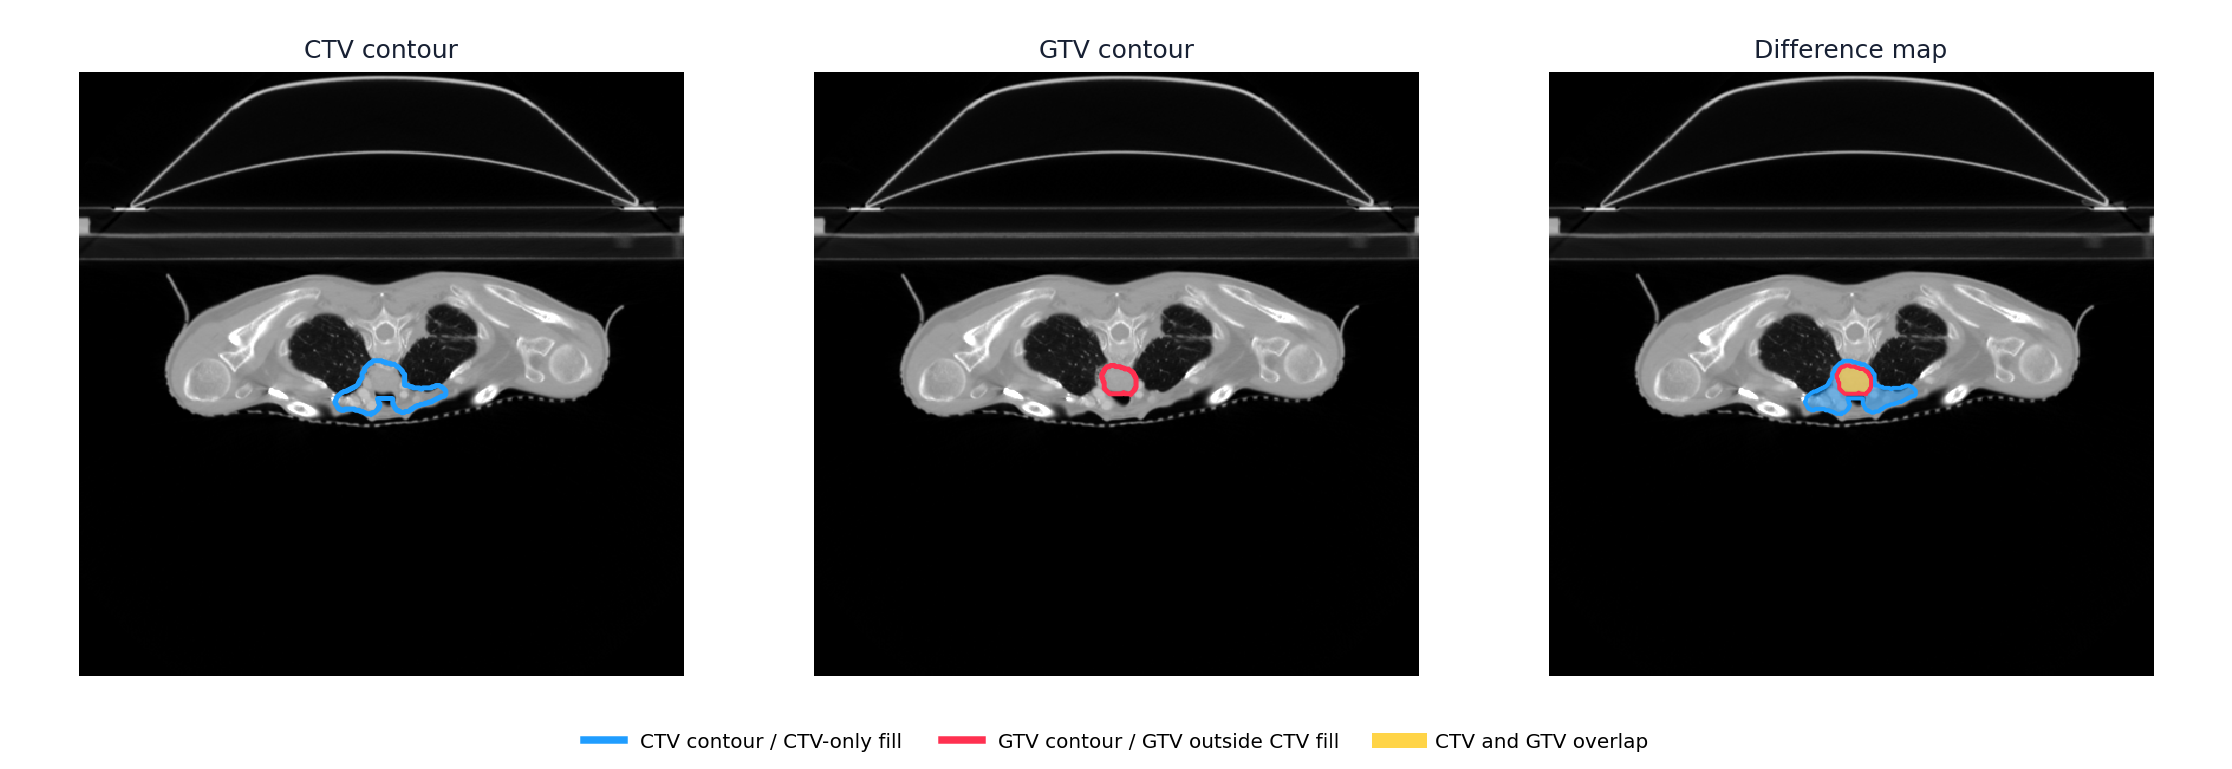
\includegraphics[width=\linewidth]{gtv_ctv_difference_example.png}
  \caption{Illustrative GTV/CTV target-hierarchy example from the separate audit subset. Blue denotes CTV-only region, yellow denotes CTV--GTV overlap, and red denotes GTV outside the CTV. The example shows that CTV is a clinically expanded target concept rather than a CT-visible tumor mask; this motivates using sparse clinician CTV prompts and anatomical priors instead of treating CTV delineation as ordinary CT-to-GTV object segmentation.}
  \label{fig:gtv-ctv-difference}
\end{figure}

Let $I\in\mathbb{R}^{Z\times H\times W}$ denote the planning CT, $A$ the OAR mask or anatomical context, $P$ the sparse CTV prompt mask, and $\Ygt$ the complete expert CTV. In retrospective evaluation, $K=7$ prompt slices are sampled from non-empty expert CTV slices to simulate a clinician providing full 2D CTV masks on representative axial slices. At test time, only $I$, $A$, and $P$ are available to the algorithm; $\Ygt$ is hidden until metric computation.

\subsection{Sparse prompt preprocessing and OAR-derived refinement ROI}

The first stage constructs a geometric pseudo-target from the sparse CTV prompts. OAR masks are then used to define a local anatomy ROI, denoted $\ROAR$, around the prompt and pseudo-target region for the refinement stage. This ROI is not used as a hard claim that OAR segmentation drives the pseudo-label Dice gain. Rather, it makes the downstream candidate region deployable and prevents the refine network from predicting freely over the whole CT volume.

For each prompted slice $z_i$, the 2D prompt mask is converted into a signed distance field:
\begin{equation}
  D_i(x,y)=\EDT(P_{z_i})(x,y)-\EDT(1-P_{z_i})(x,y),
\end{equation}
where internal voxels are positive. For unprompted slices between neighboring prompts, the SDF is interpolated along the axial direction:
\begin{equation}
  D_z(x,y)=(1-t)D_i(x,y)+tD_{i+1}(x,y),\qquad
  t=\frac{z-z_i}{z_{i+1}-z_i}.
\end{equation}
Outside the prompted range, shrinkage-controlled extrapolation is used. Multiple SDF candidates are generated by varying shrinkage and propagation settings. Their voxelwise support map is
\begin{equation}
  S(v)=\frac{1}{M}\sum_{m=1}^M \mathbb{I}[v\in Y_m],
\end{equation}
where $Y_m$ is the $m$-th SDF candidate.

The support map defines a high-confidence core $C$, a high-recall envelope $E$, and an uncertain region $U$:
\begin{equation}
  C=\{v:S(v)\geq \tau_C\}\cup P,\qquad
  E_{\mathrm{SDF}}=\{v:S(v)\geq \tau_E\},\qquad
  E=E_{\mathrm{SDF}}\cap \ROAR,\qquad
  U=E\setminus C .
\end{equation}
Prompt slices are always enforced as foreground. A train-calibrated support-intersection rule selects a pseudo-label $\Yp$ from strict SDF support and linear-core intersection candidates. The reported pseudo-label score evaluates this deployable geometric support-intersection output. In the full method, $\Yp$ is then combined with the OAR-derived ROI to form the constrained input region for the supervised refine network, rather than being treated as the final updated result.

\subsection{Supervised pseudo-to-true refine network}

The proposed refine model is a lightweight residual 3D U-Net. It is trained across historical cases and is not a one-patient-one-model method. The input tensor is
\begin{equation}
  X=[I,\Yp,C,E,P,S,A_{\mathrm{spinal}},\ROAR,d_z],
\end{equation}
where $d_z$ encodes normalized axial distance to the nearest prompted slice. The network $f_\theta$ predicts an inclusion probability map:
\begin{equation}
  p_\theta(v)=\sigma(f_\theta(X)_v).
\end{equation}
The final test-time mask is constrained by the prompt and envelope:
\begin{equation}
  \Yfinal = P \cup \left(\{v:p_\theta(v)\geq \tau\}\cap E\right),
\end{equation}
with the intended structural constraint
\begin{equation}
  C \subseteq \Yfinal \subseteq E
\end{equation}
up to the empirically learned correction behavior and prompt preservation. The probability threshold $\tau$ is selected on the validation split only. The supervised training target is the complete expert CTV $\Ygt$; the pseudo-label is never used as the target label for training.

Training uses masked binary cross-entropy and Dice losses inside the candidate region:
\begin{equation}
  \mathcal{L}=\mathcal{L}_{\mathrm{BCE}}(p_\theta,\Ygt;M)+
  \lambda \mathcal{L}_{\mathrm{Dice}}(p_\theta,\Ygt;M),
\end{equation}
where $M$ is the union of the envelope, prompt, and target foreground in the training crop. During inference, $M$ is not required; predictions are clipped by the envelope and prompt constraint. The complete preprocessing-to-refinement workflow is summarized in Fig.~\ref{fig:workflow}, and the refine-network input structure is shown in Fig.~\ref{fig:network}.

\begin{figure}[t]
  \centering
  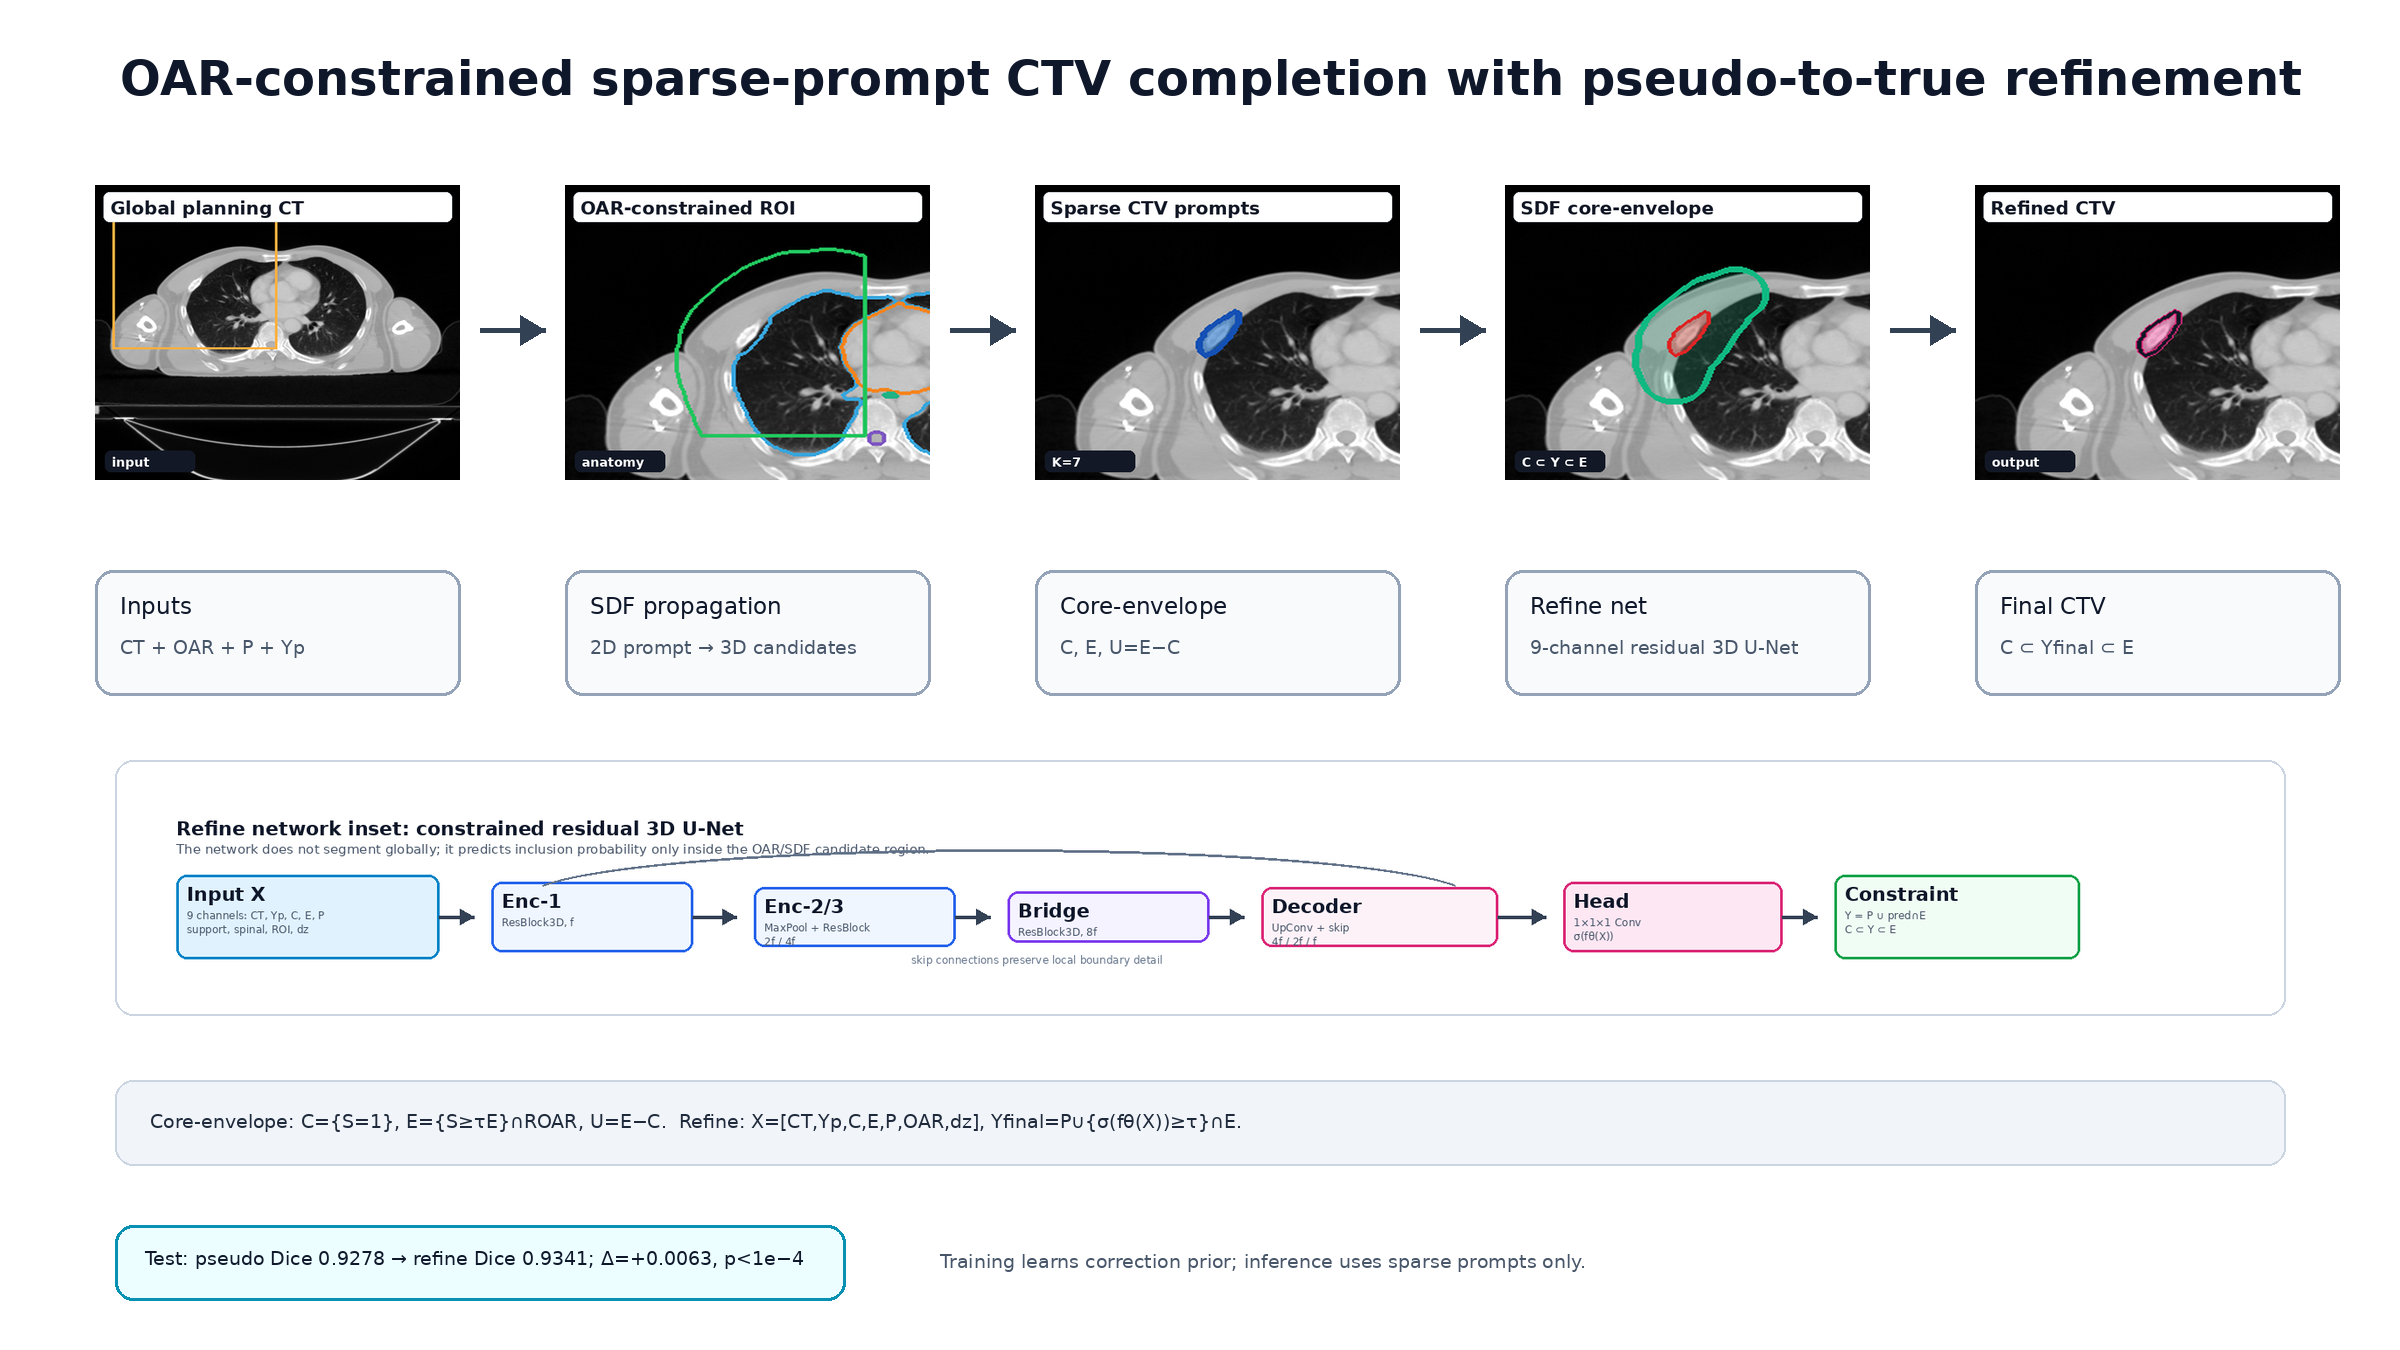
\includegraphics[width=\linewidth]{workflow_with_network.png}
  \caption{Complete workflow. Global planning CT and OAR masks define the anatomical context. Sparse CTV slice prompts are propagated by SDF candidates into a core-envelope prior and support-intersection pseudo-label. A supervised residual 3D U-Net then learns pseudo-to-true correction while the final output remains constrained by the prompt and candidate envelope.}
  \label{fig:workflow}
\end{figure}

\begin{figure}[t]
  \centering
  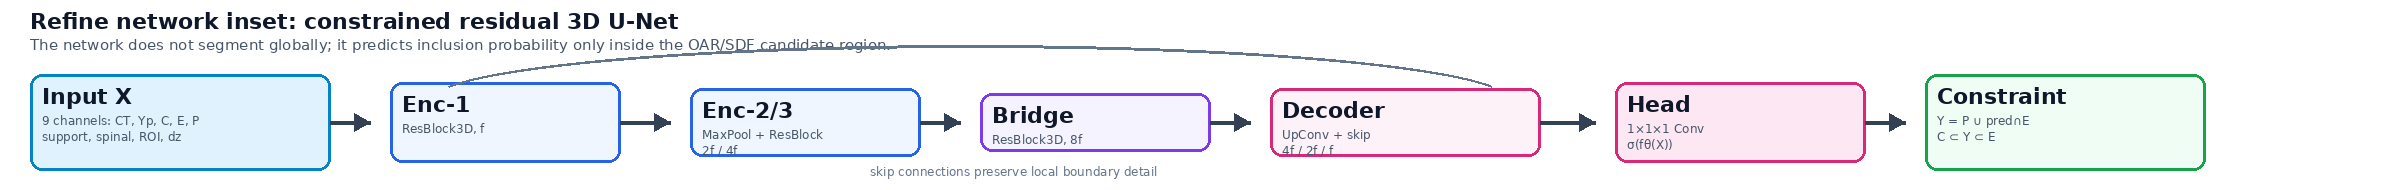
\includegraphics[width=\linewidth]{refine_network_architecture.png}
  \caption{Refine network inset. The 9-channel input combines CT, pseudo-label, SDF core, SDF envelope, prompt, support, OAR hard context, anatomy ROI, and prompt-distance channels. The residual 3D U-Net predicts an inclusion probability map inside the OAR/SDF candidate region.}
  \label{fig:network}
\end{figure}

\section{Experiments}

\subsection{Baselines}

We compare against three groups of baselines. First, no-prompt fully automatic CTV segmentation is evaluated using nnU-Net and DiffUNet. Second, promptable segmentation is evaluated using SAM-Med3D with CT-derived automatic prompts and with the same $K=7$ sparse target prompts. Third, sparse-prompt geometric preprocessing baselines include linear mask interpolation, SDF propagation, SDF core output, and the support-intersection pseudo-label used as the input to the refine network.

The comparison is intentionally strict. Linear interpolation uses exactly the same seven full-slice CTV prompts and is a strong geometry-only comparator. Therefore, the proposed method must demonstrate improvement over both conventional automatic segmentation and the strong prompt-interpolation baseline.

\subsection{Metrics and statistics}

We report Dice, unseen-slice Dice, HD95, ASD, precision, recall, and volume difference. Unseen-slice Dice excludes prompted slices and evaluates true three-dimensional completion rather than prompt copying:
\begin{equation}
  \Dice_{\mathrm{unseen}}=
  \Dice\left(\Yfinal|_{z\notin Z_P},\Ygt|_{z\notin Z_P}\right).
\end{equation}
Paired statistical tests compare the proposed refine output with the input pseudo-label on the same 31 test scans. We report paired $t$-test, Wilcoxon signed-rank test, sign test, bootstrap confidence interval for mean $\Delta$Dice, and Cohen's $d_z$.

\section{Results}

\subsection{CTV segmentation and completion performance}

\begin{table}[t]
\centering
\caption{CTV segmentation and sparse-prompt completion performance.}
\label{tab:main-ctv-results}
\begin{threeparttable}
\resizebox{\linewidth}{!}{
\begin{tabular}{@{}lllcccc@{}}
\toprule
Setting & Method & Test-time target information & DSC & uDSC & HD95 (mm) & ASD (mm) \\
\midrule
\multicolumn{7}{@{}l}{\textit{Fully automatic segmentation}} \\
No prompt & nnU-Net 3D full-resolution & None & $0.400 \pm 0.345$ & -- & $56.94 \pm 60.13$ & $33.72 \pm 45.44$ \\
No prompt & DiffUNet & None & $0.316 \pm 0.301$ & -- & $71.89 \pm 60.11$ & $41.44 \pm 44.67$ \\
\addlinespace[2pt]
\multicolumn{7}{@{}l}{\textit{Promptable foundation-model baselines}} \\
Automatic prompt & SAM-Med3D, CT-derived prompt & CT heuristic prompt & $0.157 \pm 0.187$ & -- & $85.70 \pm 36.47$ & $49.64 \pm 31.77$ \\
Sparse prompt & SAM-Med3D, sparse target prompt & $K=7$ target slices & $0.422 \pm 0.159$ & -- & $21.32 \pm 9.23$ & $5.54 \pm 3.06$ \\
\addlinespace[2pt]
\multicolumn{7}{@{}l}{\textit{Same-prompt geometric preprocessing}} \\
Sparse prompt & Linear mask interpolation & $K=7$ target slices & $0.912 \pm 0.048$ & $0.876 \pm 0.057$ & $3.90 \pm 1.66$ & $1.22 \pm 0.66$ \\
Sparse prompt & SDF propagation & $K=7$ target slices & $0.916 \pm 0.045$ & $0.871 \pm 0.064$ & $4.43 \pm 1.58$ & $1.20 \pm 0.46$ \\
Sparse prompt & SDF core & $K=7$ target slices & $0.920 \pm 0.045$ & $0.879 \pm 0.061$ & $4.21 \pm 1.58$ & $1.13 \pm 0.46$ \\
Sparse prompt & Support-intersection pseudo-label & $K=7$ target slices & $0.928 \pm 0.050$ & $0.897 \pm 0.062$ & $3.43 \pm 1.68$ & $0.97 \pm 0.54$ \\
\addlinespace[2pt]
\multicolumn{7}{@{}l}{\textit{Proposed supervised pseudo-to-true correction}} \\
Sparse prompt & \textbf{Ours: OAR/SDF-constrained refine network} & $K=7$ target slices & $\mathbf{0.934 \pm 0.045}$ & $\mathbf{0.906 \pm 0.054}$ & $\mathbf{3.11 \pm 1.37}$ & $\mathbf{0.84 \pm 0.48}$ \\
\bottomrule
\end{tabular}
}
\begin{tablenotes}[flushleft]\footnotesize
\item DSC: Dice similarity coefficient. uDSC: Dice computed after excluding the prompted slices. Values are mean $\pm$ standard deviation over 31 CTV-positive test scans. All sparse-prompt rows use the same seven full-slice CTV prompts at test time. The proposed network uses the support-intersection pseudo-label, SDF core-envelope prior, OAR-derived ROI, and sparse prompts as input; complete expert CTVs are used only for supervised training and final evaluation.
\end{tablenotes}
\end{threeparttable}
\end{table}


Table~\ref{tab:main-ctv-results} shows that fully automatic CTV segmentation is unstable in this cohort. nnU-Net achieves $0.400\pm0.345$ Dice and DiffUNet achieves $0.316\pm0.301$. SAM-Med3D with automatic CT-derived prompts reaches only $0.157\pm0.187$, and sparse-prompt SAM-Med3D reaches $0.422\pm0.159$. These results confirm that generic automatic and promptable segmentation methods do not solve the current CTV task.

The same-prompt linear interpolation baseline is much stronger, reaching $0.912\pm0.048$ Dice. This confirms that sparse full-slice CTV prompts already contain substantial patient-specific target geometry. SDF propagation and core extraction improve the structured pseudo-label to $0.916$ and $0.920$ Dice, respectively. The support-intersection pseudo-label reaches $0.9278$ Dice and $0.897$ unseen-slice Dice. The proposed supervised refine network further improves the final output to $0.9341$ Dice, $0.9057$ unseen-slice Dice, $3.11$ mm HD95, and $0.84$ mm ASD. Figure~\ref{fig:method-visual-comparison} provides a qualitative example showing the same ranking visually on an unseen slice.

\begin{figure}[t]
  \centering
  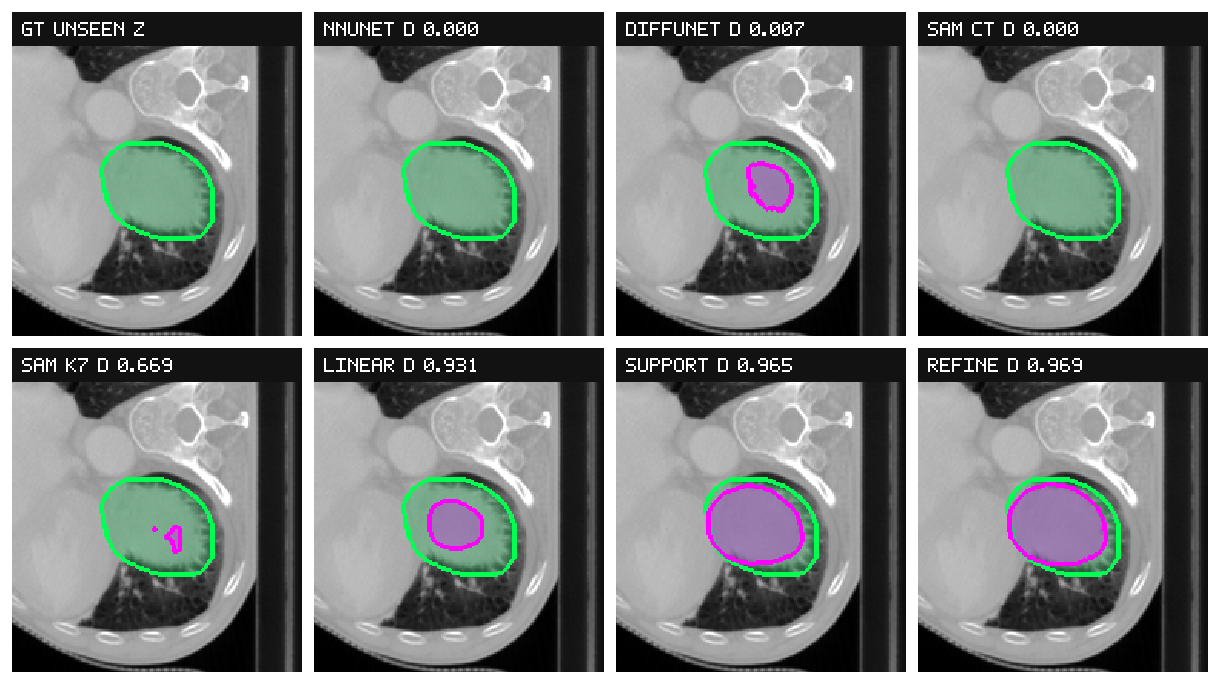
\includegraphics[width=\linewidth]{method_visual_comparison_example.png}
  \caption{Qualitative method comparison on a representative unseen slice. Green denotes the expert CTV, magenta denotes the method prediction, and the displayed $D$ value is the whole-case Dice similarity coefficient. The no-prompt networks and CT-derived SAM-Med3D prompt fail to localize the target in the CTV region, sparse-prompt SAM-Med3D undersegments the target, and linear interpolation captures only part of the volume. The support-intersection pseudo-label and the final refine-network output are visually closer to the expert contour.}
  \label{fig:method-visual-comparison}
\end{figure}

\subsection{Refine-network contribution}

\begin{table}[t]
\centering
\caption{Paired test-set evidence for the refine-network gain over the pseudo-label.}
\label{tab:refine-statistics}
\begin{threeparttable}
\begin{tabular}{@{}llc@{}}
\toprule
Evidence type & Measurement & Value \\
\midrule
\multicolumn{3}{@{}l}{\textit{Primary paired comparison on 31 held-out scans}} \\
Input & Pseudo-label DSC & $0.9278 \pm 0.0505$ \\
Output & Refined DSC & $0.9341 \pm 0.0453$ \\
Gain & Mean paired $\Delta$DSC & $+0.0063 \pm 0.0076$ \\
Gain & Median paired $\Delta$DSC & $+0.0076$ \\
Direction & Improved / worsened scans & 25 / 6 \\
\addlinespace[2pt]
\multicolumn{3}{@{}l}{\textit{Significance of the paired gain}} \\
Parametric test & Paired $t$-test, one-sided & $p=3.46\times 10^{-5}$ \\
Rank test & Wilcoxon signed-rank, one-sided & $p=4.33\times 10^{-5}$ \\
Direction test & Sign test, one-sided & $p=4.39\times 10^{-4}$ \\
Bootstrap & 95\% CI for mean $\Delta$DSC & $[0.0037,\ 0.0090]$ \\
Standardized effect & Cohen's $d_z$ & $0.829$ \\
\bottomrule
\end{tabular}
\begin{tablenotes}[flushleft]\footnotesize
\item DSC: Dice similarity coefficient. The table is intentionally limited to paired test-set evidence because the refine network is evaluated by whether it improves its own input pseudo-label on the same scans. The checkpoint (epoch 60) and probability threshold (0.70) were selected on the validation split before test evaluation; test labels were used only for the metrics and paired tests reported here.
\end{tablenotes}
\end{threeparttable}
\end{table}


Table~\ref{tab:refine-statistics} is designed as a paired evidence table rather than as a general performance table. Its purpose is to answer whether the refine network improves the exact pseudo-label that it receives as input on the same held-out scans. The input pseudo-label reaches $0.9278\pm0.0505$ Dice, and the refined output reaches $0.9341\pm0.0453$ Dice, giving a mean paired gain of $+0.0063$ with 25 improved scans and 6 worsened scans. The one-sided paired $t$-test gives $p=3.46\times10^{-5}$ and the one-sided Wilcoxon test gives $p=4.33\times10^{-5}$. The bootstrap 95\% confidence interval for the mean Dice gain is $[0.0037,0.0090]$. These results support that the observed improvement is not simply a metric fluctuation. Nevertheless, because the current formal training uses one random seed, a multi-seed robustness analysis remains an important next validation step.

\begin{table}[t]
\centering
\caption{Progressive component ablation of sparse-prompt CTV completion.}
\label{tab:ablation-summary}
\begin{threeparttable}
\resizebox{\linewidth}{!}{
\begin{tabular}{@{}clcccccc@{}}
\toprule
Step & Variant & Full-slice prompt & SDF support & Core/envelope & Supervised refine & DSC & uDSC \\
\midrule
1 & Linear mask interpolation & \checkmark & -- & -- & -- & $0.912 \pm 0.048$ & $0.876 \pm 0.057$ \\
2 & SDF propagation & \checkmark & \checkmark & -- & -- & $0.916 \pm 0.045$ & $0.871 \pm 0.064$ \\
3 & SDF core & \checkmark & \checkmark & \checkmark & -- & $0.920 \pm 0.045$ & $0.879 \pm 0.061$ \\
4 & Support-intersection pseudo-label & \checkmark & \checkmark & \checkmark & -- & $0.928 \pm 0.050$ & $0.897 \pm 0.062$ \\
5 & \textbf{Ours: pseudo-to-true refine network} & \checkmark & \checkmark & \checkmark & \checkmark & $\mathbf{0.934 \pm 0.045}$ & $\mathbf{0.906 \pm 0.054}$ \\
\bottomrule
\end{tabular}
}
\begin{tablenotes}[flushleft]\footnotesize
\item The table is ordered by the workflow rather than by unrelated parameter sweeps. Step 4 is the input pseudo-label used by the network. Step 5 adds supervised cohort-level pseudo-to-true correction without patient-specific training at test time.
\end{tablenotes}
\end{threeparttable}
\end{table}


The ablation summary in Table~\ref{tab:ablation-summary} clarifies the progression of the method. The large jump over fully automatic networks comes from sparse clinical prompts. SDF propagation and support-intersection preprocessing then provide an auditable pseudo-label. The supervised refine network gives the final improvement by learning systematic pseudo-to-true corrections from historical complete CTVs. Figure~\ref{fig:ablation-visual-progression} shows how these steps change the same target region.

\begin{figure}[t]
  \centering
  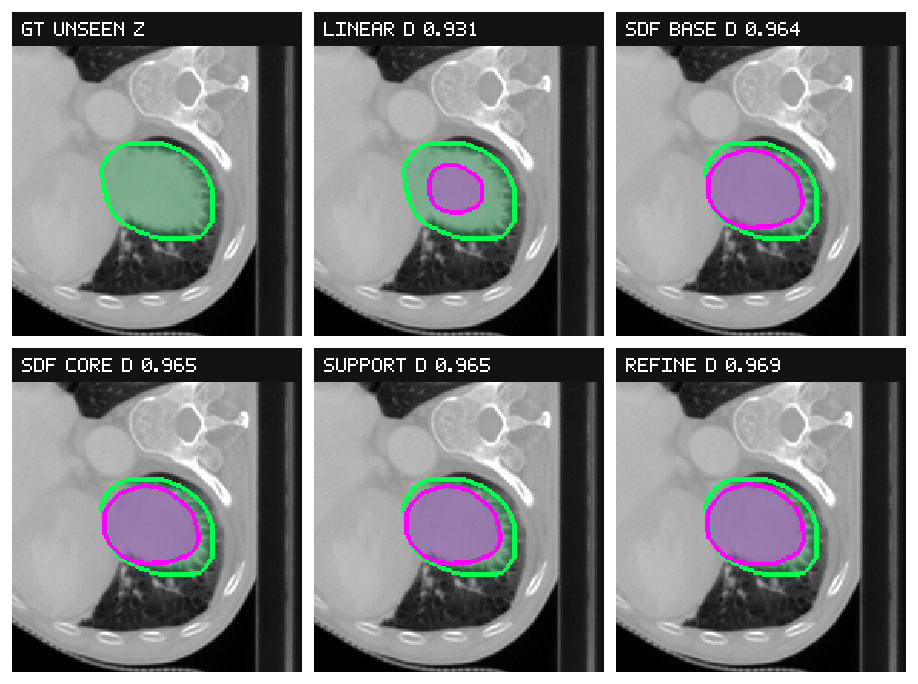
\includegraphics[width=0.88\linewidth]{ablation_visual_progression_example.png}
  \caption{Qualitative visualization of the progressive ablation on the same unseen slice as Fig.~\ref{fig:method-visual-comparison}. Green denotes the expert CTV and magenta denotes each intermediate prediction. Linear interpolation undercovers the posterior extent, SDF propagation and the SDF core move the candidate closer to the target, the support-intersection pseudo-label provides the high-quality network input, and supervised pseudo-to-true refinement gives the final correction.}
  \label{fig:ablation-visual-progression}
\end{figure}

\subsection{Auxiliary OAR segmentation}

\begin{table}[t]
\centering
\caption{Auxiliary OAR segmentation used for deployable anatomical context.}
\label{tab:oar-context-results}
\begin{threeparttable}
\begin{tabular}{@{}lcccc@{}}
\toprule
 & \multicolumn{2}{c}{nnU-Net} & \multicolumn{2}{c}{DiffUNet} \\
\cmidrule(lr){2-3}\cmidrule(lr){4-5}
Organ & DSC & HD95 (mm) & DSC & HD95 (mm) \\
\midrule
Lung & $0.976 \pm 0.021$ & $3.50 \pm 2.48$ & $0.970 \pm 0.021$ & $4.69 \pm 2.96$ \\
Heart & $0.913 \pm 0.175$ & $7.10 \pm 6.14$ & $0.894 \pm 0.174$ & $8.71 \pm 7.40$ \\
Spinal cord & $0.872 \pm 0.195$ & $16.89 \pm 61.71$ & $0.846 \pm 0.106$ & $11.33 \pm 34.82$ \\
Esophagus & $0.820 \pm 0.174$ & $4.48 \pm 4.99$ & $0.635 \pm 0.168$ & $9.57 \pm 9.14$ \\
\bottomrule
\end{tabular}
\begin{tablenotes}[flushleft]\footnotesize
\item OAR segmentation defines the anatomical ROI and safety context for CTV completion. The OAR module is reported as an auxiliary deployability component rather than as the primary CTV-performance driver.
\end{tablenotes}
\end{threeparttable}
\end{table}


OAR segmentation is evaluated because deployable inference requires an anatomical ROI. Table~\ref{tab:oar-context-results} shows that nnU-Net provides strong automatic OAR masks for lung, heart, spinal cord, and esophagus, while DiffUNet serves as an additional comparator. These OAR masks support the ROI and safety constraint, but the CTV gain is primarily driven by sparse target prompts, SDF support, and supervised pseudo-to-true correction.

Figure~\ref{fig:oar-visual-comparison} provides a qualitative OAR comparison on one representative test scan. The automatic nnU-Net and DiffUNet predictions align well with large organs such as lung and heart, whereas promptable SAM-Med3D variants are less stable for this multi-organ OAR setting. The SAM-Med3D full-GT prompt column is included as a diagnostic oracle and is not used as a fair deployable baseline.

\begin{figure}[p]
  \centering
  \setlength{\tabcolsep}{2pt}
  \renewcommand{\arraystretch}{1.04}
  \scriptsize
  \begin{tabular}{@{}lccccc@{}}
  \toprule
  Organ & GT & nnU-Net & DiffUNet & SAM CT prompt & SAM oracle \\
  \midrule
  Lung &
  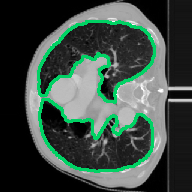
\includegraphics[width=0.155\linewidth]{oar_example_lung_GT.png} &
  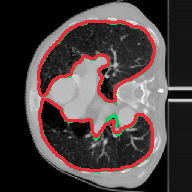
\includegraphics[width=0.155\linewidth]{oar_example_lung_nnunet.png} &
  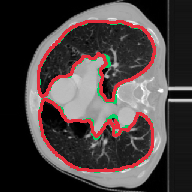
\includegraphics[width=0.155\linewidth]{oar_example_lung_diffunet.png} &
  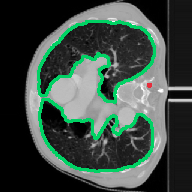
\includegraphics[width=0.155\linewidth]{oar_example_lung_sam_ct.png} &
  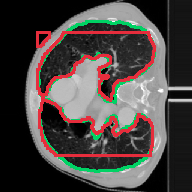
\includegraphics[width=0.155\linewidth]{oar_example_lung_sam_oracle.png} \\
  Heart &
  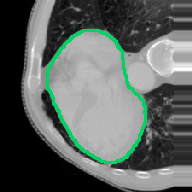
\includegraphics[width=0.155\linewidth]{oar_example_heart_GT.png} &
  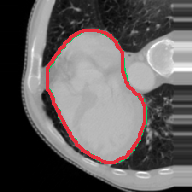
\includegraphics[width=0.155\linewidth]{oar_example_heart_nnunet.png} &
  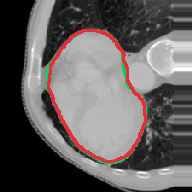
\includegraphics[width=0.155\linewidth]{oar_example_heart_diffunet.png} &
  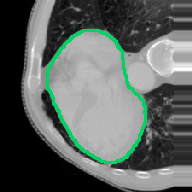
\includegraphics[width=0.155\linewidth]{oar_example_heart_sam_ct.png} &
  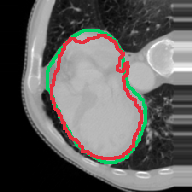
\includegraphics[width=0.155\linewidth]{oar_example_heart_sam_oracle.png} \\
  Spinal cord &
  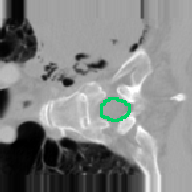
\includegraphics[width=0.155\linewidth]{oar_example_spinal_GT.png} &
  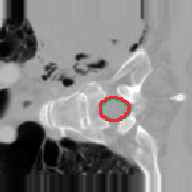
\includegraphics[width=0.155\linewidth]{oar_example_spinal_nnunet.png} &
  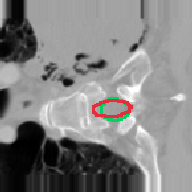
\includegraphics[width=0.155\linewidth]{oar_example_spinal_diffunet.png} &
  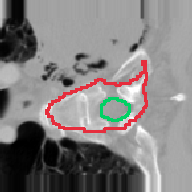
\includegraphics[width=0.155\linewidth]{oar_example_spinal_sam_ct.png} &
  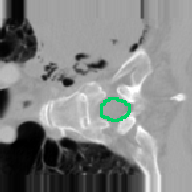
\includegraphics[width=0.155\linewidth]{oar_example_spinal_sam_oracle.png} \\
  Esophagus &
  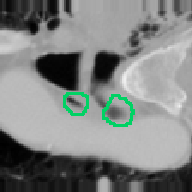
\includegraphics[width=0.155\linewidth]{oar_example_esophagus_GT.png} &
  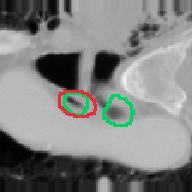
\includegraphics[width=0.155\linewidth]{oar_example_esophagus_nnunet.png} &
  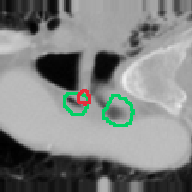
\includegraphics[width=0.155\linewidth]{oar_example_esophagus_diffunet.png} &
  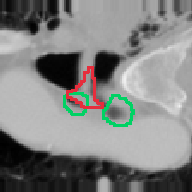
\includegraphics[width=0.155\linewidth]{oar_example_esophagus_sam_ct.png} &
  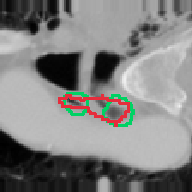
\includegraphics[width=0.155\linewidth]{oar_example_esophagus_sam_oracle.png} \\
  \bottomrule
  \end{tabular}
  \caption{Qualitative OAR segmentation comparison on a representative test scan. In all method panels, green denotes the expert OAR boundary and red denotes the method prediction boundary. The oracle SAM-Med3D column uses GT-derived prompts and is shown only as a diagnostic reference.}
  \label{fig:oar-visual-comparison}
\end{figure}

\section{Discussion}

The main finding is that sparse CTV prompts are more informative for this radiotherapy target than CT appearance alone. Fully automatic networks and generic SAM-style prompting underperform because the CTV boundary is not a visible object boundary. A same-prompt linear interpolation baseline is already strong, which is clinically meaningful: when a physician provides seven complete CTV slices, simple geometric completion captures much of the volume. The value of the proposed method is therefore not merely that it beats weak automatic baselines, but that it improves a strong sparse-prompt pseudo-label in a controlled and auditable way.

The supervised refine network changes the methodological positioning relative to a pure single-patient preprocessing method. The preprocessing stage remains patient-specific and prompt-driven, but the refine model learns cohort-level physician or institution-specific correction patterns from complete historical CTVs. At inference, the method still requires only sparse CTV prompts for the new patient and performs no patient-specific training. This positioning is more defensible than claiming that a single test case can learn the full CTV distribution.

The OAR ROI plays a different role from a primary segmentation driver. OAR masks restrict the search region and supply anatomical context, but the current evidence suggests that CTV Dice is mainly determined by prompt geometry, SDF support, and learned pseudo-to-true correction. This is advantageous for clinical transparency: OARs define where the algorithm is allowed to search, while the target prompts and SDF priors determine the CTV completion.

The work also clarifies the special-issue framing. The data are CT-based and should not be overstated as CT/MRI/PET multimodal imaging. The appropriate claim is biomedical data preprocessing: integrating imaging, anatomical contours, sparse human annotations, and distance-field representations into a pattern-recognition pipeline that produces a high-quality pseudo-label and downstream refined CTV.

Limitations include the single-institution cohort, scan-level rather than fully patient-external validation, and the current one-seed refine-network result. Some test cases with very high pseudo-label Dice were slightly worsened by the network, indicating that future models should use residual add/delete heads, stronger identity preservation, or uncertainty gating. Multi-seed training, patient-grouped validation, and external CTV datasets would strengthen the evidence before clinical deployment.

\section{Conclusion}

We presented a sparse-prompt CTV completion framework with OAR-conditioned supervised pseudo-to-true refinement. The method transforms seven clinician-approved CTV slices into an SDF core-envelope pseudo-label and then refines it with a lightweight residual 3D U-Net conditioned on CT, OAR-derived ROI context, prompt, SDF support, core, envelope, and prompt-distance channels. On 31 held-out CTV-positive scans, the proposed network improves the input pseudo-label from $0.9278$ to $0.9341$ Dice with significant paired gains. The result supports the value of combining sparse clinical prompts, structured geometric preprocessing, anatomical search constraints, and supervised refinement for difficult CTV data preprocessing.

\section*{Funding}

Funding information should be completed by the authors. If no specific funding supported this work, the statement recommended by the journal can be used: This research did not receive any specific grant from funding agencies in the public, commercial, or not-for-profit sectors.

\section*{Ethics statement}

This retrospective study uses de-identified institutional radiotherapy data. Ethics approval, consent waiver information, and data-use permission details should be completed by the authors according to institutional requirements before submission.

\section*{CRediT authorship contribution statement}

Yanxin Huang: Conceptualization, Methodology, Software, Formal analysis, Investigation, Visualization, Writing - original draft. Additional author roles, including Supervision, Resources, Funding acquisition, and Writing - review and editing, should be completed before submission.

\section*{Declaration of competing interest}

The authors declare that they have no known competing financial interests or personal relationships that could have appeared to influence the work reported in this paper.

\section*{Data availability}

The clinical CT, OAR, and CTV contours used in this study are from a private institutional radiotherapy cohort and cannot be publicly released in their raw form because of patient privacy and institutional data-governance restrictions. Derived anonymized metrics, analysis scripts, and non-identifying figure assets can be shared subject to institutional approval.

\section*{Declaration of generative AI and AI-assisted technologies in the manuscript preparation process}

During the preparation of this initial draft, AI-assisted writing and coding tools were used to help organize experimental results, draft text, and generate editable LaTeX source. The authors must review, verify, and edit all content, references, and numerical claims before submission and take full responsibility for the final manuscript.

\bibliographystyle{elsarticle-num}
\bibliography{references}

\end{document}
